\chapter{Arquitectura Software con Zenoh y ROS2}
\label{cap:capitulo4}

\begin{flushright}
\begin{minipage}[]{10cm}
\emph{Quizás algún fragmento de libro inspirador...}\\
\end{minipage}\\

Autor, \textit{Título}\\
\end{flushright}

\vspace{1cm}

%Escribe aquí un párrafo explicando brevemente lo que vas a contar en este capítulo. En este capítulo (y quizás alguno más) es donde, por fin, describes detalladamente qué has hecho y qué experimentos has llevado a cabo para validar tus desarrollos.

Este capítulo describe la topografía de red utilizada, tanto a nivel de
\textit{hardware} como a nivel de \textit{software}.
También se describe la manera en la que dichos \textit{softwares} se
complementan, detallando los aspectos más importantes de cada uno de ellos, y
explicando como funcionan juntos a nivel de \textit{software}.



\section{Topología hardware}
\label{sec:topologia_hw}

%párrafo sobre la topología harware de red
La topología de red utilizada comprende varias máquinas, debido a la naturaleza
multirobótica de este trabajo, correspondiendo todas ellas a excepción del
\textit{router}, a los ordenadores de a bordo de los robots utilizados, siendo
el \textit{router} el encargado de establecer comunicaciones entre el resto de
máquinas y encaminar así los datos que se envían entre ellas.
\\

%párrafo sobre el router a nivel harware y configuración (software).
Comenzando con el \textit{router}, no se ha necesitado una conexión a internet,
ya que las comunicaciones se han realizado de manera local, es decir, que todos
los ordenadores de abordo en los robots se comunican directamente con dicho
\textit{router}, sin necesidad de mandar datos más allá de esta red local,
dado que todos se encuentran en la misma sala, al alcance de un único
\textit{router}.
Asimismo dicho \textit{router} debe estar configurado de manera que permita la
comunicación en ambos sentidos (entrante y saliente), y debe permitirla a través
de los protocolos DDS, para los nodos de ROS2 y Zenoh, para los nodos de
Zenoh-Flow.
\\

%párrafo sobre los ordenadores de a bordo de los robots.
Los ordenadores de a bordo deben tener una mínima capacidad de cómputo como para
no saturarse a la hora de enviar o recibir una gran cantidad de mensajes.
En nuestro caso se ha utilizado el ordenador portátil mencionado en la Sección
\ref{sec:a_bordo} del capítulo anterior.
Puesto que se necesitan más ordenadores para realizar los experimentos, y solo
se dispone de un ordenador portátil, también se han utilizado las máquinas del
modelo Raspberry Pi 4B mencionadas en la sección referenciada.
\\

\begin{figure} [h!]
  \begin{center}
    \includegraphics[width=8cm]{figs/network_topology}
  \end{center}
  \caption{Topología de red centralizada.}
  \label{fig:network_topology}
\end{figure}\

El ordenador portátil se ha utilizado en conjunto con el robot Turtlebot 2,
mostrado en la Sección \ref{sec:turtlebot2}, mientras que las Raspberry Pi 4B es
utilizada en los propios robots Turtlebot 4, mostrados en la Sección
\ref{sec:turtlebot4}, a modo de ordenador de a bordo interno.
\\

Dado que el portátil es el ordenador más potente utilizado, este deberá correr
todo el software relativo a Zenoh-Flow, además de estar conectado al robot, como
se puede ver representado en la Figura \ref{fig:network_topology}.
\\



\section{Topología software}
\label{sec:topologia_sw}

%párrafo sobre los ordenadores de a bordo de los robots.
A nivel de \textit{software}, aparte de la configuración del \textit{router}
mencionada anteriormente, se ha necesitado ejecutar un \textit{router} de Zenoh
y un \textit{bridge} de Zenoh en cada robot, permitiendo de esta manera las
comunicaciones en ambos sentidos entre ellos y a su vez la utilización de los
protocolos Zenoh y DDS al mismo tiempo.
Las máquinas utilizadas también necesitan una configuración de red para poder
operar con estas herramientas \textit{software}.
\\

Además, nuestra topología será centralizada, lo que quiere decir que una de las
máquinas, llamada ordenador principal o centralizado, correrá todo el
\textit{software} desarrollado en Zenoh-Flow, por lo que deberá tener instalado
dicho \textit{software} además del \textit{router} y el bridge de Zenoh.
La máquina elegida para este propósito será consecuentemente la que mayor
capacidad de cómputo tiene, que en este caso es el portátil, como se ha
mencionado en la Sección \ref{sec:topologia_hw}.


\subsection{Zenoh-bridge-DDS}
\label{sec:zenoh_bridge}

Como ya se ha mencionado previamente, este \textit{software} permite traducir
las comunicaciones entre Zenoh y DDS, en ambas direcciones, estableciendo un
puente entre ellas, como su nombre indica.
Gracias a esta propiedad del \textit{bridge} y a la posibilidad de serializar
los mensajes en el interior de los nodos de Zenoh-Flow, utilizando la misma
función que se usa internamente en ROS2 para serializarlos, se puede establecer
una comunicación directa entre nodos de Zenoh-Flow y de ROS2 en ambas
direcciones y a pesar de utilizar distintos protocolos.
\\

Esto nos permite seguir utilizando las funcionalidades existentes programadas
en ROS2, a la vez que desarrollar código compatible en Zenoh-Flow que utilice
dichas funcionalidades sin ningún impedimento, como se verá más adelante en la
Sección \ref{sec:zenoh_flow}.
\\


\subsection{Zenoh-Flow}
\label{sec:zenoh_flow}

Zenoh-Flow es un \textit{framework} diseñado para la programación de flujos de
datos, que funciona sobre el protocolo Zenoh, y que se puede comunicar a través
de DDS con nodos de ROS gracias al Zenoh-bridge-DDS como queda explicado en la
Sección \ref{sec:zenoh_bridge}.
Esta capacidad nos permite hacer uso de nodos de ROS en los flujos de datos, así
como realizar aplicaciones robóticas directamente en conjunto con nodos de ROS,
como se explica más adelante en esta sección.
\\

Para la programación de flujos de datos con este \textit{framework} es necesario
la definición de un flujo de datos, en un archivo en formato \texttt{yaml}, como
el que podemos ver en el Código de ejemplo \ref{cod:data_flow_example}, que
puede encontrarse en el repositorio oficial de ejemplos de Zenoh-Flow\footnote{
\url{https://github.com/ZettaScaleLabs/zenoh-flow-examples/blob/master/getting-started}}.
\\

% Con esta linea no funciona (para usar la definición comentada en estilo.tex):
%\begin{lstlisting}[language=yaml]
\begin{code}[H]
  \begin{lstlisting}[style=yaml]
    flow: getting-started

    vars:
     BASE_DIR: "/path/to/zenoh-flow-examples/getting-started"
    
    sources:
      - id: zenoh-sub
        configuration:
          key-expressions:
            out: zf/getting-started/hello
        descriptor: "builtin://zenoh"
    
    operators:
      - id: greetings-maker
      descriptor: "file://{{ BASE_DIR }}/nodes/python/greetings-maker/greetings-maker.yaml"
    
    sinks:
      - id: file-writer
      descriptor: "file://{{ BASE_DIR }}/nodes/python/file-writer/file-writer.yaml"
    
      - id: zenoh-writer
        configuration:
          key-expressions:
            in: zf/getting-started/greeting
        descriptor: "builtin://zenoh"
    
    links:
      - from:
          node: zenoh-sub
          output: out
        to:
          node: greetings-maker
          input: name
    
      - from:
          node: greetings-maker
          output: greeting
        to:
          node: file-writer
          input: in
    
      - from:
          node: greetings-maker
          output: greeting
        to:
          node: zenoh-writer
          input: in
  \end{lstlisting}
\caption[Definición de flujo de datos en Zenoh-Flow]{Definición de flujo de datos en Zenoh-Flow}
\label{cod:data_flow_example}
\end{code}

%Párrafo sobre las etiquetas importantes del código.
En el contenido de este archivo pueden verse varios apartados importantes, como
son: las variables de configuración que recibirán los nodos, denominada con la
etiqueta \verb|vars|; la definición de los distintos nodos con las etiquetas
\verb|source|, \verb|operator| o \verb|sink|, donde se definen las rutas los
archivos \texttt{yaml} que los describen, incluyendo sus entradas, salidas o
variables de configuración, como se explicarán a continuación; y las conexiones
entre ellos con la etiqueta \verb|links|, en cuyo interior se define la entradas
y salidas de cada nodo a conectar.
\\

%Párrafo sobre las etiquetas importantes que no están en el código.
Además, se puede añadir la etiqueta \verb|mapping|, donde se especifica en qué
máquina correrá cada nodo, aunque en nuestro caso no será necesario debido a que
todos los nodos correrán en el mismo ordenador (el más potente), para liberar
capacidad de cómputo a los demás.
De esta manera, nuestra topología será centralizada.
\\

%Párrafo sobre los descriptores builtin o integrados.
En este ejemplo se puede ver cómo los nodos \verb|zenoh-sub| y
\verb|zenoh-writer|, contienen la línea \verb|descriptor: "builtin://zenoh"|, lo
que indica que no necesitan un fichero que describa dónde se encuentra el código
de dicho nodo, ya que este se encuentra directamente integrado en Zenoh-Flow, y
lo que harán será recibir y información de la \textit{key-expression}
\verb|zf/getting-started/hello| y publicar información a la
\textit{key-expression} \verb|zf/getting-started/greeting| respectivamente, como
puede observarse resumidamente en la Figura \ref{fig:zf_example}.
\\

%Párrafo sobre los descriptores no integrados.
El resto de nodos deben ser programados, para lo que existe un fichero
descriptor, que indicará el nombre del nodo, las variables de configuración, la
ruta al archivo de código del propio nodo y los nombres de sus \textit{inputs} y
\textit{outputs}.
Continuando con el mismo ejemplo, se muestran en el Código
\ref{cod:node_descriptor} las propiedades mencionadas, en este caso del nodo
\textit{operator} con el nombre \verb|greetings-maker|, que consecuentemente se
encontrará en la ruta declarada en su etiqueta \verb|descriptor|.
\\

\begin{code}[H]
  \begin{lstlisting}[style=yaml]
    id: greetings-maker
    vars:
      BASE_DIR: "/path/to/zenoh-flow-examples/getting-started"
    uri: "file://{{ BASE_DIR }}/nodes/python/greetings-maker/greetings-maker.py"
    inputs: [name]
    outputs: [greeting]
  \end{lstlisting}
\caption[Fichero de descriptor de un nodo de Zenoh-Flow]{Fichero de descriptor de un nodo de Zenoh-Flow}
\label{cod:node_descriptor}
\end{code}

\begin{figure} [h!]
  \begin{center}
    \includegraphics[width=5cm]{figs/zenoh_flow_example}
  \end{center}
  \caption{Flujo de datos de ejemplo en Zenoh-Flow.}
  \label{fig:zf_example}
\end{figure}\

%Párrafo sobre las partes del código del nodo operator de ejemplo.
Las distintas partes del código de este nodo se muestran en el Código
\ref{cod:operator_node}, en el que puede verse cómo se reduce a una sencilla
clase que hereda de la clase del nodo en cuestión, en este caso de la clase
\verb|Operator|. Además debe existir una función externa \verb|register()| que
debe devolver la clase creada para este nodo, en nuestro caso llamada
\verb|GreetingsMaker|.
\\

La programación de los nodos de Zenoh-Flow, realizada en \texttt{Python}, es muy
parecida entre los distintos nodos, ya que su funcionamiento es muy similar: los
nodos \textit{source} solo comprenden salidas de datos, los nodos \textit{sink},
solo comprenden entradas, y los nodos \textit{operator} comprenden ambas, ya que
pueden recibir información de otros nodos \textit{source} u \textit{operator} y
pueden enviar datos a otros nodos \textit{operator} o \textit{sink}, como
podemos ver en el flujo de datos representado en la anterior Figura
\ref{fig:zf_example} o en la Figura \ref{fig:data_flow_qr_example} de la Sección
\ref{sec:flujos_datos}.
\\

\begin{code}[H]
  \begin{lstlisting}[language=Python]
    from zenoh_flow.interfaces import Operator
    from zenoh_flow import Inputs, Outputs
    from zenoh_flow.types import Context
    from typing import Dict, Any
    
    class GreetingsMaker(Operator):
        def __init__(
            self,
            context: Context,
            configuration: Dict[str, Any],
            inputs: Inputs,
            outputs: Outputs,
        ):
            self.output = outputs.take("greeting", str, lambda s: bytes(s, "utf-8"))
            self.in_stream = inputs.take("name", str, lambda buf: buf.decode("utf-8"))
            if self.in_stream is None:
                raise ValueError("No input 'name' found")
            if self.output is None:
                raise ValueError("No output 'greeting' found")
    
        def finalize(self) -> None:
            return None
    
        async def iteration(self) -> None:
            message = await self.in_stream.recv()
            name = message.get_data()
            if name is not None:
                greetings = self.generate_greetings(name)
                await self.output.send(greetings)
            return None
    
        def generate_greetings(self, name: str) -> str:
            greetings_dict = {
                "Sofia": "Ciao, {}!\n",
                "Gabriele": "Ciao, PaaS manager!\n",
            }
            greet = greetings_dict.get(name, "Hello, {}!\n")
            return greet.format(name)
    
    def register():
        return GreetingsMaker
  \end{lstlisting}
\caption[Fichero de código de un nodo \texttt{operator} en Zenoh-Flow]{Fichero de código de un nodo \texttt{operator} de Zenoh-Flow}
\label{cod:operator_node}
\end{code}



%Párrafos sobre la función constructor (__init__()) de la clase del nodo.
La línea \verb|outputs.take("greeting", str, lambda s: bytes(s, "utf-8"))|, en
la función constructor de esta clase (\verb|__init__()|), toma como argumentos
el nombre del \textit{output}, el tipo de mensaje, y la función que utilizará
para serializar el mensaje en el momento de enviarlo, devolviendo el
\textit{output} correspondiente.
Lo mismo sucede con la línea siguiente, aunque esta toma como tercer argumento
una función que utilizará para deserializar el mensaje en el momento en el que
sea recibido.
Esta línea devolverá el \textit{input} que corresponda.
Son estas funciones las que se deberán sustituir por las análogas de ROS, si se
quiere enviar o recibir información de los nodos de ROS con ayuda del
\textit{bridge}, como ya se ha explicado anteriormente.
\\

Además, en esta como en cualquier otra clase de \texttt{Python} se pueden
declarar las variables necesarias a la hora de desarrollar el \textit{software}.
Teniendo en cuenta que la variable \verb|configuration| es un diccionario, las
distintas variables de configuración especificadas en los archivos anteriores,
pueden ser obtenidas con una línea como
\verb|configuration.get(conf_var_name, default)|, en la que se deberá
especificar el nombre de la variable en cuestión en forma de cadena de
caracteres o \texttt{str} en el primer argumento, y será devuelto el valor
asociado a dicha clave.
\\

%Párrafo sobre la función finalize() de la clase del nodo.
Dentro de esta clase existe una función llamada \verb|finalize()| que se
ejecutará antes de destruir el nodo, por lo que aquí se podrá liberar memoria,
cerrar o ventanas abiertas o creadas por el nodo o cualquier otra funcionalidad
que se requiera finalizar.
\\

%Párrafo sobre la función finalize() de la clase del nodo.
Por último, tenemos la función más importante, llamada \verb|iteration()|, que
deberá ser asíncrona para poder recibir mensajes, y lo hará ejecutando el método
\verb|recv()| del \textit{input} en cuestión como se ve en la línea
\verb|await self.in_stream.recv()|, lo cual deserializará el dato y lo devolverá
cuando este llegue.
Esa misma función permitirá realizar los cálculos y tomar las decisiones que se
necesiten, para mandar los datos resultantes de manera similar, esta vez usando
el método \verb|send()| del output por el que se desee enviar, como sucede con
la línea \verb|await self.output.send(greetings)|, con lo que, finalmente,
podemos deducir la función que realizará este nodo: publicará una frase de
bienvenida que variará en función del nombre que reciba.
Esta función se repetirá iterativamente hasta finalizar el flujo de datos.
\\



\subsection{Flujos de datos con Zenoh-Flow y ROS2}
\label{sec:zf_ros}
%[TODO] Explicar cómo publicar o recibir desde ROS, explicando detalles como
%       "rt/topic_name...", los bridge y router, etc (añadir la imagen
%       siguiente):
Como ya se ha visto, Zenoh-Flow divide sus posibles nodos en tres tipos:
\textit{source}, \textit{operator} y \textit{sink}, que podríamos trasladar a
las palabras en español: origen, operador y final, pudiendo ver la relación de
estos nodos con un grafo direccionado, como es un flujo de datos, en el que
los datos se obtienen de los nodos origen o \textit{source}, pasan por el
operador, en el que son computados, o tratados, hasta llegar al final o
\textit{source}, donde los datos dejan de viajar entre nodos para terminar
convirtiéndose en una acción o decisión del sistema.
Ya se ha visto representada esta misma comparación en la Figura
\ref{fig:data_flow_vs_robotics} de la Sección \ref{sec:flujos_datos}.

Para poder complementar los explicados flujos de datos en Zenoh-Flow con las
acciones de los robots, que se ejecutan en nodos de ROS2, se deben crear las
piezas faltantes, para anclar ambos sistemas, uniendo sus entradas y salidas.
Entre estas piezas se encuentran el serializador y el deserializador, que como
se ha explicado previamente, debe ser el mismo utilizado internamente en ROS.
\\

Esto resulta en el Código \ref{cod:zf_ros_serializer}, en el que se pueden
observar dos funciones: la primera, \verb|ser_ros2_msg()|, en la que se
serializa el mensaje en su primer argumento y la segunda, que en cambio devuelve
una función creada en el momento y que deserializará el mensaje en función de su
tipo, especificado en su primer argumento.
Esto debe hacerse de esta manera ya que no podemos saber el tipo de mensaje que
se recibirá, ya que estará serializado en bytes, a diferencia de cuando se
envía, momento en el que se tiene el tipo de mensaje, con la ayuda de la función
\verb|type()| de \texttt{Python}.
\\

\begin{code}[H]
  \begin{lstlisting}[language=Python]
    from rclpy.impl.implementation_singleton import rclpy_implementation as _rclpy
    from rclpy.type_support import check_for_type_support

    def ser_ros2_msg(ros2_msg) -> bytes:
        check_for_type_support(type(ros2_msg))
        return _rclpy.rclpy_serialize(ros2_msg, type(ros2_msg))

    def get_ros2_deserializer(ros2_type): # Returns a function
        check_for_type_support(ros2_type)
        return lambda obj: _rclpy.rclpy_deserialize(obj, ros2_type)
  \end{lstlisting}
\caption[Funciones para serializar y deserializar mensajes de ROS en Zenoh-Flow]{Funciones para serializar y deserializar mensajes de ROS en Zenoh-Flow}
\label{cod:zf_ros_serializer}
\end{code}

Estas dos funciones, serán especificadas en los argumentos de nuestros nodos de
Zenoh-Flow a la hora de obtener las entradas y salidas, definiendo de esta
manera al sistema, el método a seguir para serializar y deserializar los
mensajes de ROS, como se puede ver en el Código \ref{cod:ros_zf_io}.
\\

\begin{code}[H]
  \begin{lstlisting}[language=Python]
    from zenoh_flow.interfaces import Operator
    from zenoh_flow import Input, Output
    from zenoh_flow.types import Context
    from typing import Dict, Any
    from geometry_msgs.msg import PoseStamped
    from tf2_msgs.msg import TFMessage

    class Navigator(Operator):
        def __init__(
            self,
            context: Context,
            configuration: Dict[str, Any],
            inputs: Dict[str, Input],
            outputs: Dict[str, Output],
        ):
            inputs.take("TF1", TFMessage, deserializer=get_ros2_deserializer(TFMessage))
            outputs.take("RobotPose1", PoseStamped, serializer=ser_ros2_msg)
            ...
        ...
  \end{lstlisting}
\caption[Serializador/deserializador en los input/output de un nodo Zenoh-Flow]{Serializador/deserializador en el input/output de un nodo Zenoh-Flow}
\label{cod:ros_zf_io}
\end{code}

La siguiente pieza del puzle, consiste en configurar el \textit{bridge} de
Zenoh, para que únicamente traduzca el tráfico deseado, lo que conseguiremos con
un argumento en la línea de comandos al ejecutarlo, o bien utilizando
\texttt{--allow/-a} seguido de un \textit{string} que contenga los topics
deseados (o partes de los mismos), separados por el carácter ``\texttt{|}'', o
bien utilizando \texttt{--deny/-d} de la misma manera, lo que traducirá todos
los topics excepto los que contengan los \textit{strings} especificados.
Un ejemplo del comando de ejecución con este argumento es el siguiente:
\begin{lstlisting}[language=bash]
  ./zenoh-bridge-dds -e tcp/<ip>:7447 --allow "goal_pose|zf/getting-started/"
\end{lstlisting}
%\verb+./zenoh-bridge-dds -e tcp/<ip>:7447 --allow "goal_pose|zf/getting-started/"+,
siendo el argumento \texttt{-e} y el siguiente, la configuración de conexión del
\textit{bridge}, debiéndose sustituir \verb|<ip>| por la dirección IP a la que
se quiera conectar, como se verá más adelante en el Capítulo
\ref{cap:capitulo5}.
Un esquema explicativo de toda esta sección puede verse en la Figura
\ref{fig:zenoh_dds_topology}.
\\
%Nota: \verb++ evita e caracteres como "|" sean interpretados.

\begin{figure} [h!]
  \begin{center}
    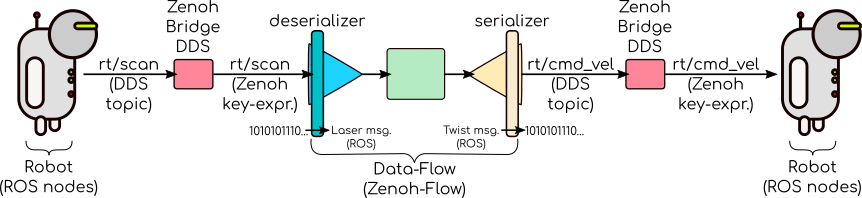
\includegraphics[width=15cm]{figs/zenoh_dds_topology}
  \end{center}
  \caption{Topología software con ROS (DDS) y Zenoh-Flow (Zenoh).}
  \label{fig:zenoh_dds_topology}
\end{figure}\











